\section{MEASURE ZERO AND CONTENT ZERO}
A subset $A$ of Rn has ($n$-dimensional) \textbf{measure} 0 if for every
$\varepsilon > 0$ there is a cover $\{U_1, U_2, U_3, \cdots \}$ of $A$ by 
closed rectangles such that $\sum_{i=1}^{\infty}{v(U_i)}< \varepsilon$.
It is obvious (but nevertheless useful to remember) that if $A$ has measure 0 and
$B \subset A$, then $B$ has measure 0.
The reader may verify that open rectangles may be used instead of closed rectangles in
the definition of measure 0.

A set with only finitely many points clearly has measure 0.
If A has infinitely many points which can be arranged in a
sequence $a_1, a_2, a_3,\cdots$, then $A$ also has measure 0, 
for if $\varepsilon>0$, we can choose $U_i$ to be closed rectangle
containing $a_i$ with $v(U_i)< \varepsilon/2^i$. Then 
$\sum_{i=1 }^{\infty}{v(U_i)} < \sum_{i=1 }^{\infty}{\varepsilon/2^i} = \varepsilon$.

The set of all rational numbers between 0 and 1 is an impor-
tant and rather surprising example of an infinite set whose
members can be arranged in such a sequence.
To see that this is so, list the fractions in the following array in the order
indicated by the arrows (deleting repetitions and numbers
greater than 1):

\begin{figure}[H]
    \centering
    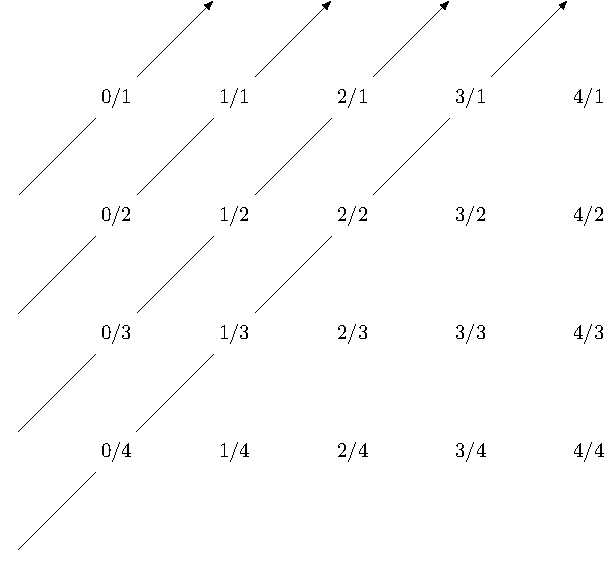
\includegraphics[width=.65\linewidth]{./pics/Fig3-(1).pdf}
\end{figure}

An important generalization of this idea can be given.

\begin{theorem}
    If $A = A_1\cup A_2 \cup A_3\cup \cdots$ and each $A_i$ has measure 0, then $A$ has measure 0.
\end{theorem}

\begin{proof}
    Let $\varepsilon>0$. Since $A_i$ has measure 0, there is a cover $\{U_{i,1}, U_{i,2}, U_{i,3}, \cdots \}$ 
    of $A_i$ by closed rectangles such that $\sum_{j=1}^{\infty}{v(U_{i,j})}< \varepsilon/2^i$. 
    Then the collection of all $\{U_{i,j}\}$ is a cover of $A$. By consider the array
    \begin{figure}[!htb]
        \centering
        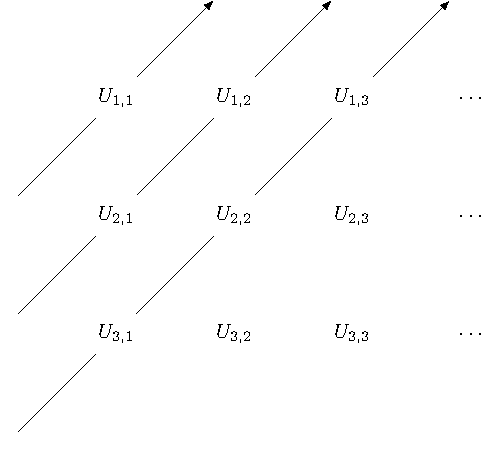
\includegraphics[width=.6\linewidth]{./pics/Fig3-(2).pdf}
    \end{figure}
\end{proof}

we see that this collection can be arranged in a sequence  
$V_1, V_2, V_3,\cdots$. Clearly $\sum_{i=1}^{\infty}{v(U_i)}
<\sum_{i=1}^{\infty}{\varepsilon/2^i}<\varepsilon$

A subset $A$ of $\B{R}^n$ has ($n$-dimensional) \textbf{content} 0 if for every 
$\varepsilon>0$ there is a finite cover $\{U_1, \cdots, U_n\}$ of $A$ by closed 
rectangles such that $\sum_{i=1}^{n}{v(U_i)}<\varepsilon$. If $A$ has content 0,
then $A$ clearly has measure 0. Again, open rectangles could be used instead of 
closed rectangles in the definition.

\begin{theorem}
    If $a<b$, then $[a, b]\subset \B{R}$ does not have content 0.
    In fact, if $\{U_1, \cdots, U_n\}$ is any finite cover of $[a, b]$ by closed
    intervals, then $\sum_{i=1}^{n}{v(U_i)}\ge b-a$.  
\end{theorem}

\begin{proof}
    Clearly we can assume that each $U_i\subset [a, b]$. Let 
    $a=t_0<t_1<\cdots<t_k=b$ be all endpoints of all $U_i$.
    Then each $v(U_i)$ is the sum of certain $t_j-t_{j-1}$.
    Moreover, each $[t_{j-1}, t_j]$ lies in at least one $U_i$.
    (namely, any one which contains an  interior point of $[t_{j-1}, t_j]$),
    so $\sum_{i=1}^{n}{v(U_i)} \ge \sum_{j=1}^{n}{(t_j-t_{j-1})} = b-a$.
\end{proof}

If $a < b$, it is also true that $[a,b]$ does not have measure 0.
This follows from 
\begin{theorem}
    If $A$ is compact and has measure 0, then $A$ has content 0.
\end{theorem}

\begin{proof}
    Let $\varepsilon>0$. Since $A$ has measure 0, there is a cover 
    $\{U_1, U_2,\cdots\}$ of $A$ by open rectangles such that 
    $\sum_{i=1}^{\infty}{v(U_i)} <\varepsilon$. Since $A$ is compact,
    a finite number $U_1, \cdots, U_n$ of the $U_i$ also cover $A$
    and surely $\sum_{i=1}^{n}{v(U_i)} <\varepsilon$.
\end{proof}

The conclusion of Theorem 3-6 is false if $A$ is not compact.
For example, let $A$ be the set of rational numbers between 0
and 1; then $A$ has measure 0. Suppose, however, that 
$\{[a_1, b_1]\cup \cdots \cup [a_n,b_n]\}$ covers $A$. Then $A$
is contained in the closed set $[a_1, b_1]\cup \cdots \cup [a_n,b_n]$,and 
therefore $[0, 1]\subset [a_1, b_1]\cup \cdots \cup [a_n,b_n]$. It follows 
from Theorem 3-5 that $\sum_{i=1 }^{n }{(b_i-a_i)}\ge 1$ for any such cover, and 
consequently $A$ does not have content 0.



\begin{problems}
    \problem{
        Prove that $[a_1, b_1]\times \cdots \times [a_n,b_n]$ dose not have content 0 
        if $a_i<b_i$ for each $i$.
    }    
    \problem{
        \begin{enumerate}[label=(\alph*)]
            \item Show that an unbounded set cannot have content 0.
            \item Give an example of a closed set of measure 0 which does not
            have content 0.
        \end{enumerate}
    }
    \problem{
        \begin{enumerate}[label=(\alph*)]
            \item If $C$ is a set of content 0, show that the boundary of $C$ has
            content 0.
            \item Give an example of a bounded set $C$ of measure 0 such that
            the boundary of $C$ does not have measure 0.
        \end{enumerate}
    }
    \problem{
        Let $A$ be the set of Problem 1-18. If $\sum_{i=1}^{\infty}{(b_i-a_i)}<1$, show 
        that the boundary of $A$ dose not have measure 0.
    }
    \problem{
        Let $f:[a, b]\to \F{R}$ be an increasing function. Show that 
        $\{x: f\text{ is discontinuous at } x\}$ has measure 0.
        \textit{Hint:}Use Problem 1-30 to show that $\{x: o(f,x) > 1/n\}$ 
        is finite, for each integer $n$.
    }
    \problem[*]{
        \begin{enumerate}[label=(\alph*)]
            \item Show that the collection of all rectangles $[a_1, b_1]\times \cdots \times [a_n,b_n]$
                with all $a_i$ and $b_i$ rational can be arranged in a sequence. 
            \item If $A\subset \F{R}$ is any set and $\C{O}$ is an open cover of $A$, show that 
                there is a sequence $U_1, U_2,U_3,\cdots$ of members of $\C{O}$ which also cover 
                $A$ . \textit{Hint:} For each $x\in A$ there is rectangle $B = [a_1, b_1]\times 
                \cdots \times [a_n,b_n]$ with all $a_i$ rational such that $x\in B\subset U$ for 
                some $U\in \C{O}$.
        \end{enumerate}
    }
\end{problems}
